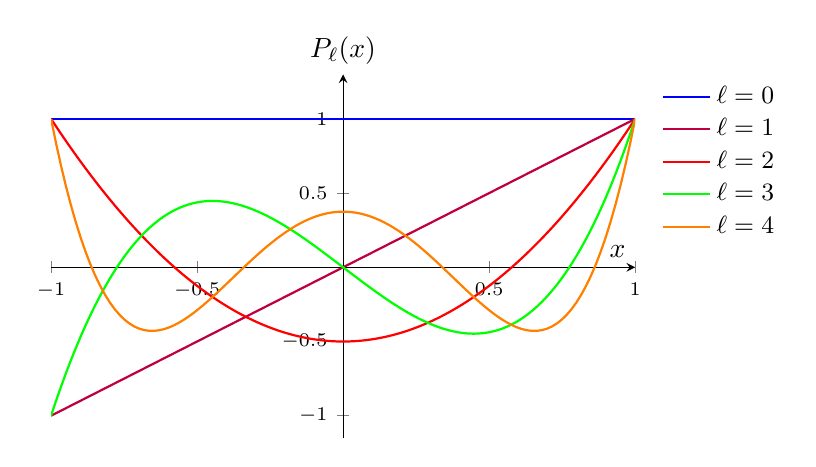
\begin{tikzpicture}
  \begin{axis}[
    width=9cm, height=6.2cm,
    xmin=-1, xmax=1, ymin=-1.15, ymax=1.3,
    axis lines=middle,
    xlabel={$x$}, ylabel={$P_\ell(x)$}, every axis y label/.style={at={(ticklabel* cs:1.0)}, anchor=south},
    xtick={-1,-0.5,0.5,1}, ytick={-1,-0.5,0.5,1},
    tick label style={font=\scriptsize},
    legend pos=outer north east,
    legend style={font=\small, draw=none},
    samples=120, domain=-1:1,
  ]
    \addplot[blue, thick] {1};
    \addlegendentry{$\ell=0$}
    \addplot[purple, thick] {x};
    \addlegendentry{$\ell=1$}
    \addplot[red, thick] {(3*x^2-1)/2};
    \addlegendentry{$\ell=2$}
    \addplot[green, thick] {(5*x^3-3*x)/2};
    \addlegendentry{$\ell=3$}
    \addplot[orange, thick] {(35*x^4-30*x^2+3)/8};
    \addlegendentry{$\ell=4$}
  \end{axis}
\end{tikzpicture}
